\section*{\textbf{Methods}}

\subsection*{Bilinear network autoregression model}

The bilinear network autoregression model provides a framework for understanding how interactions between actors in a network can be modeled over time \citep{minhas:etal:2016}. In this paper, we extend this framework by presenting the Social Influence Regression (SIR) model, which not only offers a novel method to explain the factors driving the influence parameters in the bilinear autoregression model but also introduces a more efficient estimation scheme. Our iterative block coordinate descent method dramatically accelerates the estimation process compared to the Bayesian approach originally used in the bilinear autoregression framework, making it much faster and more scalable for large networks.

Many studies examine the flows or linkages among actors, such as whether two countries are in conflict with one another. These interactions are often represented as an $n \times n$ matrix, as shown in Figure~\ref{fig:matrix}, where $n$ denotes the total number of actors in the network. We label the rows by $i$ and the columns by $j$, with $i,j \in \{1,2,\dots,n\}$. The off-diagonal elements $y_{ij}$ denote the interaction that actor $i$ directs to actor $j$. In undirected data, $y_{ij}$ may indicate, for example, whether $i$ and $j$ are allied. In directed data, the rows represent senders and the columns represent receivers, so $y_{ij}$ would indicate an action sent from $i$ to $j$. The diagonal elements $y_{ii}$ are typically undefined, indicating that actors do not interact with themselves. Although we will introduce time later (with $t=1,\ldots,T$), this figure illustrates a single snapshot of interactions at one point in time.

\begin{figure}[ht]
\centering
\begin{minipage}{.45\textwidth}
	\begin{equation*}
	Y_{t} = \bbordermatrix{
		~ & i  & \ldots & j & \ldots & k \cr
		i & NA  & \ldots & y_{ji} & \ldots & y_{ik} \cr
		\vdots & \vdots & \ddots & \vdots & \ddots & \vdots  \cr
		j & y_{ji}  & \ldots & NA  & \ldots & y_{jk} \cr
		\vdots & \vdots & \ddots & \vdots & \ddots & \vdots \cr
		k & y_{ki}  & \ldots & y_{kj}  & \ldots & NA \cr
		}
	\end{equation*}
	\caption{Matrix representation of a dyadic, relational measure for one time point.}
	\label{fig:matrix}
\end{minipage}
\begin{minipage}{0.45\textwidth}
	\centering
	\resizebox{.7\textwidth}{!}{\begin{tikzpicture}

% 	% Green
% 	\begin{scope}[xshift=1cm, yshift=1cm]
% 	\node{
% 		\begin{tikzpicture}[scale=.5]
% 			 \draw[thin, black,fill=green3] (0,0) grid (4,4) rectangle (0,0) ;
% 		\end{tikzpicture}
% 	};
% 	\end{scope}

% 	\begin{scope}[xshift=.5cm, yshift=.5cm]
% 	\node[](green){
% 		\begin{tikzpicture}[scale=.5]
% 			 \draw[thin, black,fill=green2] (0,0) grid (4,4) rectangle (0,0) ;
% 		\end{tikzpicture}
% 	} ;
% 	\end{scope}

% 	\begin{scope}
% 	\node{
% 		\begin{tikzpicture}[scale=.5]
% 			 \draw[thin, black,fill=green1] (0,0) grid (4,4) rectangle (0,0) ;
% %			\node at (3.5,3.5) { \tiny{ $y_{i j v t }$ } }; 
% 		\end{tikzpicture}
% 	};
% 	\end{scope}
	
	% Blue
	\begin{scope}[xshift=4.5cm, yshift=1cm]
	\node{
		\begin{tikzpicture}[scale=.5]
			 \draw[thin, black,fill=blue4] (0,0) grid (4,4) rectangle (0,0) ;
		\end{tikzpicture}
	};
	\end{scope}

	\begin{scope}[xshift=4cm, yshift=.5cm]
	\node[](blue){
		\begin{tikzpicture}[scale=.5]
			 \draw[thin, black,fill=blue3] (0,0) grid (4,4) rectangle (0,0) ;
		\end{tikzpicture}
	};
	\end{scope}

	\begin{scope}[xshift=3.5cm]
	\node{
		\begin{tikzpicture}[scale=.5]
			 \draw[thin, black,fill=blue2] (0,0) grid (4,4) rectangle (0,0) ;
		\end{tikzpicture}
	};
	\end{scope}
	
\end{tikzpicture}}
	\caption{Array representation of a longitudinal dyadic measure. Darker shading indicates later time periods.}
	\label{fig:tensViz}
\end{minipage}
\end{figure}

Figure~\ref{fig:matrix} captures interactions between actors at a single point in time. However, interactions are often observed over a series of time points. To represent longitudinal network data, we stack these adjacency matrices into an array, as shown in Figure~\ref{fig:tensViz}. Specifically, let $Y = \{Y_t : t = 1, \ldots, T\}$ be a time series of relational data, where $T$ represents the number of time points. The resulting array has dimensions $n \times n \times T$. The bilinear autoregression model is designed to estimate dependencies in such structures by regressing the network at one time point on its lag. The relationship between these time points is captured by a pair of matrices that reflect sender and receiver dependence patterns for each dyad.

A generalized bilinear autoregression model for $Y$ is given by:

\begin{align*}
	E [ y_{i,j,t} ] &= g( \mu_{i,j,t} ), \\
	\{ \mu_{i,j,t} \} &= M_t = A X_t B^{\top}, \\
	\{ \mu_{i,j,t} \} & = a_i^{\top} X_{t} b_j,
\end{align*}

where $x_{i,j,t}$ is a function of the lagged outcome $y_{i,j,t-1}$. For instance, we might define 
$\tilde{x}_{i,j,t} = \log(y_{i,j,t-1} + 1)$, indicating that each dyad's interaction at time $t-1$ helps predict its behavior at time $t$. 

In the application, we explore an example involving count data, where $Y$ is a time series of matrices defining count-based events between actors. For instance, we model $ y_{i,j,t} \sim \text{Poisson}(e^{\mu_{i,j,t}})$, with $ \tilde{x}_{i,j,t} = \log(y_{i,j,t-1} + 1)$. This framework is extendable to other distributions, as it is based on a generalized bilinear model. The matrices $A$ and $B$ are $n \times n$ ``influence parameters." For any pair of actors $(i,i')$, the element $a_{ii'}$ in $A$ captures how predictive the actions of country $i'$ at time $t-1$ are of the actions of country $i$ at time $t$. $b_{jj'}$ in $B$ captures how predictive the actions directed at country $j'$ at time $t-1$ are of the actions directed towards country $j$ at time $t$.

For example, in a bilinear autoregression model on conflict involving the United Kingdom (GBR) and the United States of America (USA), if $ a_{\text{GBR}, \text{USA}} $ is greater than zero, it implies that countries with which the USA initiated or continued a conflict in period $t-1$ are likely to also face conflict from GBR in period $t$. This suggests that GBR's future actions are influenced by the USA, or more concretely, the USA's actions are predictive of GBR's.

While the bilinear autoregression model provides a robust framework for capturing dependence patterns within network data, it falls short in its ability to explain the underlying mechanisms driving these influence patterns. Specifically, the model does not incorporate exogenous factors that may account for why certain actors exert influence within the network, limiting its interpretability and theoretical grounding. The Social Influence Regression (SIR) model, introduced in the next section, addresses this gap by incorporating exogenous covariates, offering a more detailed and interpretable understanding of what drives the influence parameters, $a$ and $b$, within the network. This innovation not only enhances the explanatory power of the model but also enables greather theoretical insight into the dynamics of network interactions.

\subsection*{Social influence regression}

The SIR model explains influence in terms of covariates by specifying a linear regression for the influence parameters $a_{ii'}$ and $b_{jj'}$. Specifically, to determine which characteristics of actor $i$ or $i'$ are associated with the influence parameter $a_{ii'}$, we write
\[
a_{ii'} = \alpha^{\top} w_{ii'} 
\quad \text{and} \quad
b_{jj'} = \beta^{\top} w_{jj'},
\]
where $w_{ii'}$ and $w_{jj'}$ are vectors of nodal and dyadic covariates describing the relationship between actors $i$ and $i'$, and between $j$ and $j'$, respectively. The parameter vectors $\alpha$ and $\beta$ then capture how each covariate contributes to sender- or receiver-level influence. In our application below, these covariates vary over time, so the model extends naturally to
\[
a_{ii',t} = \alpha^{\top} w_{ii',t}
\quad \text{and} \quad
b_{jj',t} = \beta^{\top} w_{jj',t},
\]
allowing exogenous attributes to change at each time point and thus shape evolving influence dynamics.

The network autoregression model can be expressed as:

\begin{align*}
	\mu_{i,j,t}  
	&= \sum_{i'=1}^{n} \sum_{j'=1}^{n} a_{i,i',t} \, x_{i',j',t} \, b_{j,j',t} 
	  \;=\; \sum_{i'=1}^{n} \sum_{j'=1}^{n} \alpha^{\top} w_{i,i',t} 
		  \, x_{i',j',t} \, w_{j,j',t}^{\top} \beta 
	\\
	&= \alpha^{\top} \biggl(\sum_{i'=1}^{n} \sum_{j'=1}^{n} 
			  x_{i',j',t}\, w_{i,i',t} \, w_{j,j',t}^{\top} 
		\biggr) 
	  \,\beta
	\;=\; \alpha^{\top} \tilde{X}_{i,j,t}\,\beta.
\end{align*}
	

Typically, $y_{i,j,t}$ also has covariates. For example, we might want to condition estimation of the parameters on a lagged version of the dependent variable, $y_{i,j,t-1}$, a measure of reciprocity, $y_{j,i,t-1}$, and other exogenous variables. In the case of estimating a model on material conflict between a pair of countries, this might include other exogenous aspects such as the geographical distance between a pair of countries. These additional exogeneous parameters can be accommodated with a model of the form:

\begin{align*}
	\mu_{i,j,t} = \theta^{\top} z_{i,j,t} +  \alpha^{\top} \tilde{X}_{ijt} \beta,
\end{align*}

where $z_{i,j,t}$ is a vector of exogenous covariates (e.g., distance or alliance status) associated with dyad $(i,j)$ at time $t$, representing parameters that may have a direct effect on the dependent variable. The model presented here is a type of low-rank matrix regression, where $y_{ij,t}$ is regressed on $X_{ij,t}$, which typically encodes relational-level predictors or prior network interactions relevant to dyad $(i,j)$ at time $t$. An unconstrained (linear) regression would be expressed as 
\[
\mu_{ij,t} = \theta^{\top} z_{ij,t} +  \langle C,  X_{ij,t} \rangle,
\]
where $C$ is an arbitrary $p\times p$ matrix of regression coefficients to be estimated. In contrast, the regression specified above restricts $C$ to be rank one, expressible as $C=\alpha \beta^{\top}$. This follows from the identity $\langle \alpha \beta^{\top}, X_{ij,t} \rangle  = \alpha^{\top} X_{ij,t} \beta$. Low-rank matrix regression models of this form have been considered by \citet{li:etal:2010} and \citet{zhou:etal:2013}.

\subsection*{Estimation}

The estimation of the parameters $\{\theta, \alpha, \beta\}$ in the bilinear network autoregression model is challenging due to the bilinear nature of the model. To address this, we employ an iterative block coordinate descent method, which alternately optimizes the parameters by treating one set of parameters as fixed while optimizing over the others. Specifically, the estimation process capitalizes on the fact that for fixed $\beta$, the model is linear in $\theta$ and $\alpha$, and for fixed $\alpha$, it is linear in $\theta$ and $\beta$. The conditional likelihood function for each of these cases can thus be optimized using standard techniques for generalized linear models (GLMs), specifically through iterative weighted least squares (IWLS).

The model can be expressed as follows:

\begin{align*}
	\mu_{i,j,t} & = ( \theta^{\top} \ \alpha^{\top} )
	\left ( \begin{array}{c} z_{i,j,t} \\ \tilde{X}_{ijt} \beta \end{array} \right ) \\
	 &= ( \theta^{\top} \ \beta^{\top} )
	\left ( \begin{array}{c} z_{i,j,t} \\ \tilde{X}_{ijt}^{\top} \alpha \end{array} \right )
\end{align*}

where $\mu_{i,j,t}$ represents the expected value of the interaction between actors $i$ and $j$ at time $t$, $z_{i,j,t}$ denotes the vector of covariates associated with the dyad $(i, j)$ at time $t$, and $\tilde{X}_{ijt}$ is the matrix of explanatory variables.

Given this setup, the parameters $\theta$, $\alpha$, and $\beta$ are estimated through the following iterative block coordinate descent procedure:

\begin{enumerate}
    \item \textbf{Initialize}: Start with an initial guess for $\beta$.
    \item \textbf{Iterate}: 
    \begin{enumerate}
        \item \textbf{Optimize $\theta$ and $\alpha$}: With $\beta$ fixed, estimate $\theta$ and $\alpha$ by maximizing the conditional log-likelihood function using iterative weighted least squares (IWLS). This is equivalent to fitting a generalized linear model (GLM) with the response variable $y$ regressed on the design matrix $\tilde{X}$, which is constructed by concatenating $z_{ij,t}$ and $X_{ij,t} \beta$ for each dyad $(i, j)$ and time $t$.
        \item \textbf{Optimize $\theta$ and $\beta$}: With $\alpha$ fixed, estimate $\theta$ and $\beta$ by maximizing the conditional log-likelihood function using IWLS. This step is analogous to step (a) but with the design matrix $\tilde{X}$ constructed by concatenating $z_{ij,t}$ and $X_{ij,t}^{\top} \alpha$.
    \end{enumerate}
    \item \textbf{Convergence}: Repeat steps (a) and (b) until the parameters converge, i.e., until the changes in the parameter estimates between iterations fall below a specified tolerance level.
\end{enumerate}

The iterative process leverages the fact that for each subproblem, the estimation reduces to a series of low-dimensional GLM optimizations. By solving these smaller problems iteratively, the overall estimation problem, which is bilinear and thus non-trivial, becomes manageable.

To implement the above steps, consider the following detailed process for step 1 (optimizing $\theta$ and $\alpha$):

\begin{enumerate}
    \item \textbf{Construct the Design Matrix}:
    \begin{enumerate}
        \item Let $\tilde{x}_{ij,t}$ be a vector of length $p+q$ obtained by concatenating $z_{ij,t}$ and $X_{ij,t} \beta$. Here, $p$ is the length of the vector $w_{ii'}$, and $q$ is the length of $z_{ij,t}$.
        \item Construct the design matrix $\tilde{X}$ with dimensions $n \times (n-1) \times T$ by $p+q$, where each row corresponds to a specific dyad $(i, j)$ at time $t$ and is equal to $\tilde{x}_{ij,t}$.
    \end{enumerate}
    \item \textbf{Create the Response Vector}:
    \begin{enumerate}
        \item Let $y$ be a vector of length $n \times (n-1) \times T$ consisting of the entries of $Y = \{ Y_1, \ldots, Y_T \}$, ordered to correspond with the rows of $\tilde{X}$.
    \end{enumerate}
    \item \textbf{Perform Poisson Regression}:
    \begin{enumerate}
        \item Obtain the MLEs for the Poisson regression of $y$ on $\tilde{X}$, which yields the conditional estimates of $\theta$ and $\alpha$.
    \end{enumerate}
    \item \textbf{Repeat for $\theta$ and $\beta$}:
    \begin{enumerate}
        \item In step 2 of the iterative algorithm, repeat the process by constructing the design matrix $\tilde{X}$ with $X_{ij,t}^{\top} \alpha$ replacing $X_{ij,t} \beta$ in step 1(a).
    \end{enumerate}
\end{enumerate}

The block coordinate descent method is particularly suited to this estimation problem because it effectively decomposes a high-dimensional optimization problem into more manageable subproblems. Each iteration refines the parameter estimates by focusing on a lower-dimensional subset of the parameters, thereby reducing the complexity of the problem.

Convergence is assessed by monitoring the change in parameter estimates across iterations. The process is typically stopped when the relative change in the log-likelihood or the parameter estimates between successive iterations falls below a predetermined threshold.\footnote{The choice of convergence criteria and initial values for $\beta$ can impact the speed and stability of convergence, and these factors are considered in the implementation of the algorithm. We will provide software in $\sf{R}$ to implement these types of models. The software will be hosted on CRAN and/or the corresponding author's github.}

The iterative nature of the estimation process ensures that the resulting parameter estimates are as close as possible to the true maximum likelihood estimates, given the bilinear structure of the model. This method provides a robust and efficient means of estimating the parameters in complex network models where direct optimization would be infeasible.

\subsection*{Inference}

After estimating the parameters of the SIR model, we assess the precision of these estimates by computing the standard errors. These standard errors are derived from the variance-covariance matrix, which is obtained from the inverse of the Hessian matrix of the log-likelihood function. Computing the standard errors, however, requires a consideration of the identifiability of the multiplicative parameters $ \alpha $ and $ \beta $.

The log-likelihood function for the SIR model, assuming a Poisson distribution for the count data, is given by:

\[
\ell(\theta, \alpha, \beta) = \sum_{i \neq j} \left( y_{ij,t} \log(\mu_{ij,t}) - \mu_{ij,t} \right),
\]

where $ \mu_{ij,t} = \exp(\eta_{ij,t}) $ and $ \eta_{ij,t} = Z_{ij,t}^\top \theta + \alpha^\top X_{ij,t} \beta $ represents the linear predictor incorporating both the fixed effects $Z_{ij,t}$ and the multiplicative terms involving the influence parameters $\alpha$ and $\beta$.

The parameters $ \alpha $ and $ \beta $ are not inherently identifiable because the term $ \alpha^\top X \beta $ is equivalent to $ \left(\frac{\alpha}{c}\right)^\top X \left(c \beta\right) $ for any scalar $ c $. To obtain meaningful derivative-based standard errors, we must first establish an identifiable parameterization of the model. This can be achieved by imposing a scale restriction on either $ \alpha $ or $ \beta $, or by fixing one element of either vector. The identifiable parameterization employed here restricts the first element of $ \alpha $ to be one, ensuring that the model parameters are uniquely determined.

The Hessian matrix $ H(\theta, \alpha, \beta) $ is composed of the second-order partial derivatives of the log-likelihood function with respect to the parameters $ \theta $, $ \alpha $, and $ \beta $, considering the identifiable parameterization:

\[
H(\theta, \alpha, \beta) = -\frac{\partial^2 \ell(\theta, \alpha, \beta)}{\partial \psi^2},
\]

where $\psi = (\theta, \alpha_{-1}, \beta)$ represents the identifiable parameter vector, excluding the fixed element of $\alpha$. For the identifiable parameterization, the Hessian matrix specifically consists of:

\[
H(\theta, \alpha, \beta) = \begin{pmatrix}
H_{\theta \theta} & H_{\theta \alpha_{-1}} & H_{\theta \beta} \\
H_{\alpha_{-1} \theta} & H_{\alpha_{-1} \alpha_{-1}} & H_{\alpha_{-1} \beta} \\
H_{\beta \theta} & H_{\beta \alpha_{-1}} & H_{\beta \beta}
\end{pmatrix},
\]

where each block is defined by the second derivatives:

\[
H_{\theta_k \theta_l} = -\sum_{i \neq j} \left( \mu_{ij,t} Z_{ij,k} Z_{ij,l} \right),
\]

\[
H_{\alpha_{ii'} \alpha_{ii''}} = -\sum_{i \neq j} \left( \mu_{ij,t} X_{i'j,t-1} \beta_{jj'} X_{i''j,t-1} \beta_{jj'} \right),
\]

\[
H_{\beta_{jj'} \beta_{jj''}} = -\sum_{i \neq j} \left( \mu_{ij,t} \alpha_{ii'} X_{i'j,t-1} \alpha_{ii'} X_{i'j'',t-1} \right).
\]

The mixed partial derivatives are:

\[
H_{\theta_k \alpha_{ii'}} = -\sum_{i \neq j} \left( \mu_{ij,t} Z_{ij,k} X_{i'j,t-1} \beta_{jj'} \right),
\]

\[
H_{\theta_k \beta_{jj'}} = -\sum_{i \neq j} \left( \mu_{ij,t} Z_{ij,k} \alpha_{ii'} X_{i'j,t-1} \right),
\]

\[
H_{\alpha_{ii'} \beta_{jj'}} = -\sum_{i \neq j} \left( \mu_{ij,t} X_{i'j,t-1} X_{i'j,t-1} \right).
\]

These expressions involve the expected counts $\mu_{ij,t} = \exp(\eta_{ij,t})$, which depend on the current estimates of $\theta$, $\alpha$, and $\beta$, and the design matrices $Z$ and $X$.

Given the identifiable parameterization, the standard errors for the parameters are derived from the inverse of the Hessian matrix:

\[
\text{Cov}(\hat{\theta}, \hat{\alpha}, \hat{\beta}) = -H^{-1}(\hat{\theta}, \hat{\alpha}, \hat{\beta}),
\]

where the standard errors are the square roots of the diagonal elements of this variance-covariance matrix:

\[
\text{SE}(\hat{\theta}_k) = \sqrt{ \left[ \text{Cov}(\hat{\theta}, \hat{\alpha}, \hat{\beta}) \right]_{kk} }.
\]

To obtain model-robust standard errors that are less sensitive to model misspecification, we employ a sandwich variance estimate:

\[
\widehat{\text{Var}}(\hat{\psi}) = H^{-1} S H^{-1},
\]

where $ S $ is the empirical information matrix, computed as:

\[
S = \sum_{i,j,t} \left( y_{i,j,t} - \mu_{i,j,t} \right) \dot{L}_{ij,t} \dot{L}_{ij,t}^\top,
\]

and $ \dot{L}_{ij,t} $ denotes the gradient (derivative) of the log-likelihood with respect to the parameters for a single observation $ y_{ij,t} $. The robust standard errors are then given by:

\[
\text{Robust SE}(\hat{\psi}_k) = \sqrt{ \left[ \widehat{\text{Var}}(\hat{\psi}) \right]_{kk} }.
\]

This robust variance-covariance matrix accounts for the variability in the score functions across observations, providing standard errors that are valid under a broader set of conditions.

Approximate standard errors and confidence intervals for the parameters are obtained from the derivatives of the log-likelihood function at the MLE. The asymptotic validity of these standard errors relies upon the assumption that the model is correctly specified. However, by using robust standard errors derived from the sandwich estimator, we ensure that the inferences drawn from the model are reliable even in the presence of potential model violations. In the application that follows in the next section, we utilize model-robust standard errors.

Figure~\ref{fig:socialInfluenceViz} provides a visual summary of this model. The array in the far left represents the network being modeled, the design array in green represents explanatory variables used to directly model linkages between dyads, and the $\theta$ vector includes the estimates of the effect those variables have on the network. To capture dependence patterns, a logged and lagged version of dependent variable are included, along with a design array containing a set of influence covariates, $W$; $\alpha$ and $\beta$ are vectors that capture parameter estimates for the effects of those influence covariates. By framing influence in a bilinear regression structure, SIR moves beyond the ``black box'' of simply noting that actors who resemble one another tend to form ties, and instead estimates how prior dyadic interactions (sender- and receiver-level) affect current interactions. A benefit of this framework is that once  estimated, linear combinations of the influence regression parameters permit visualizing the resulting sender and receiver dependence patterns in the network. 

\begin{figure}[ht]
	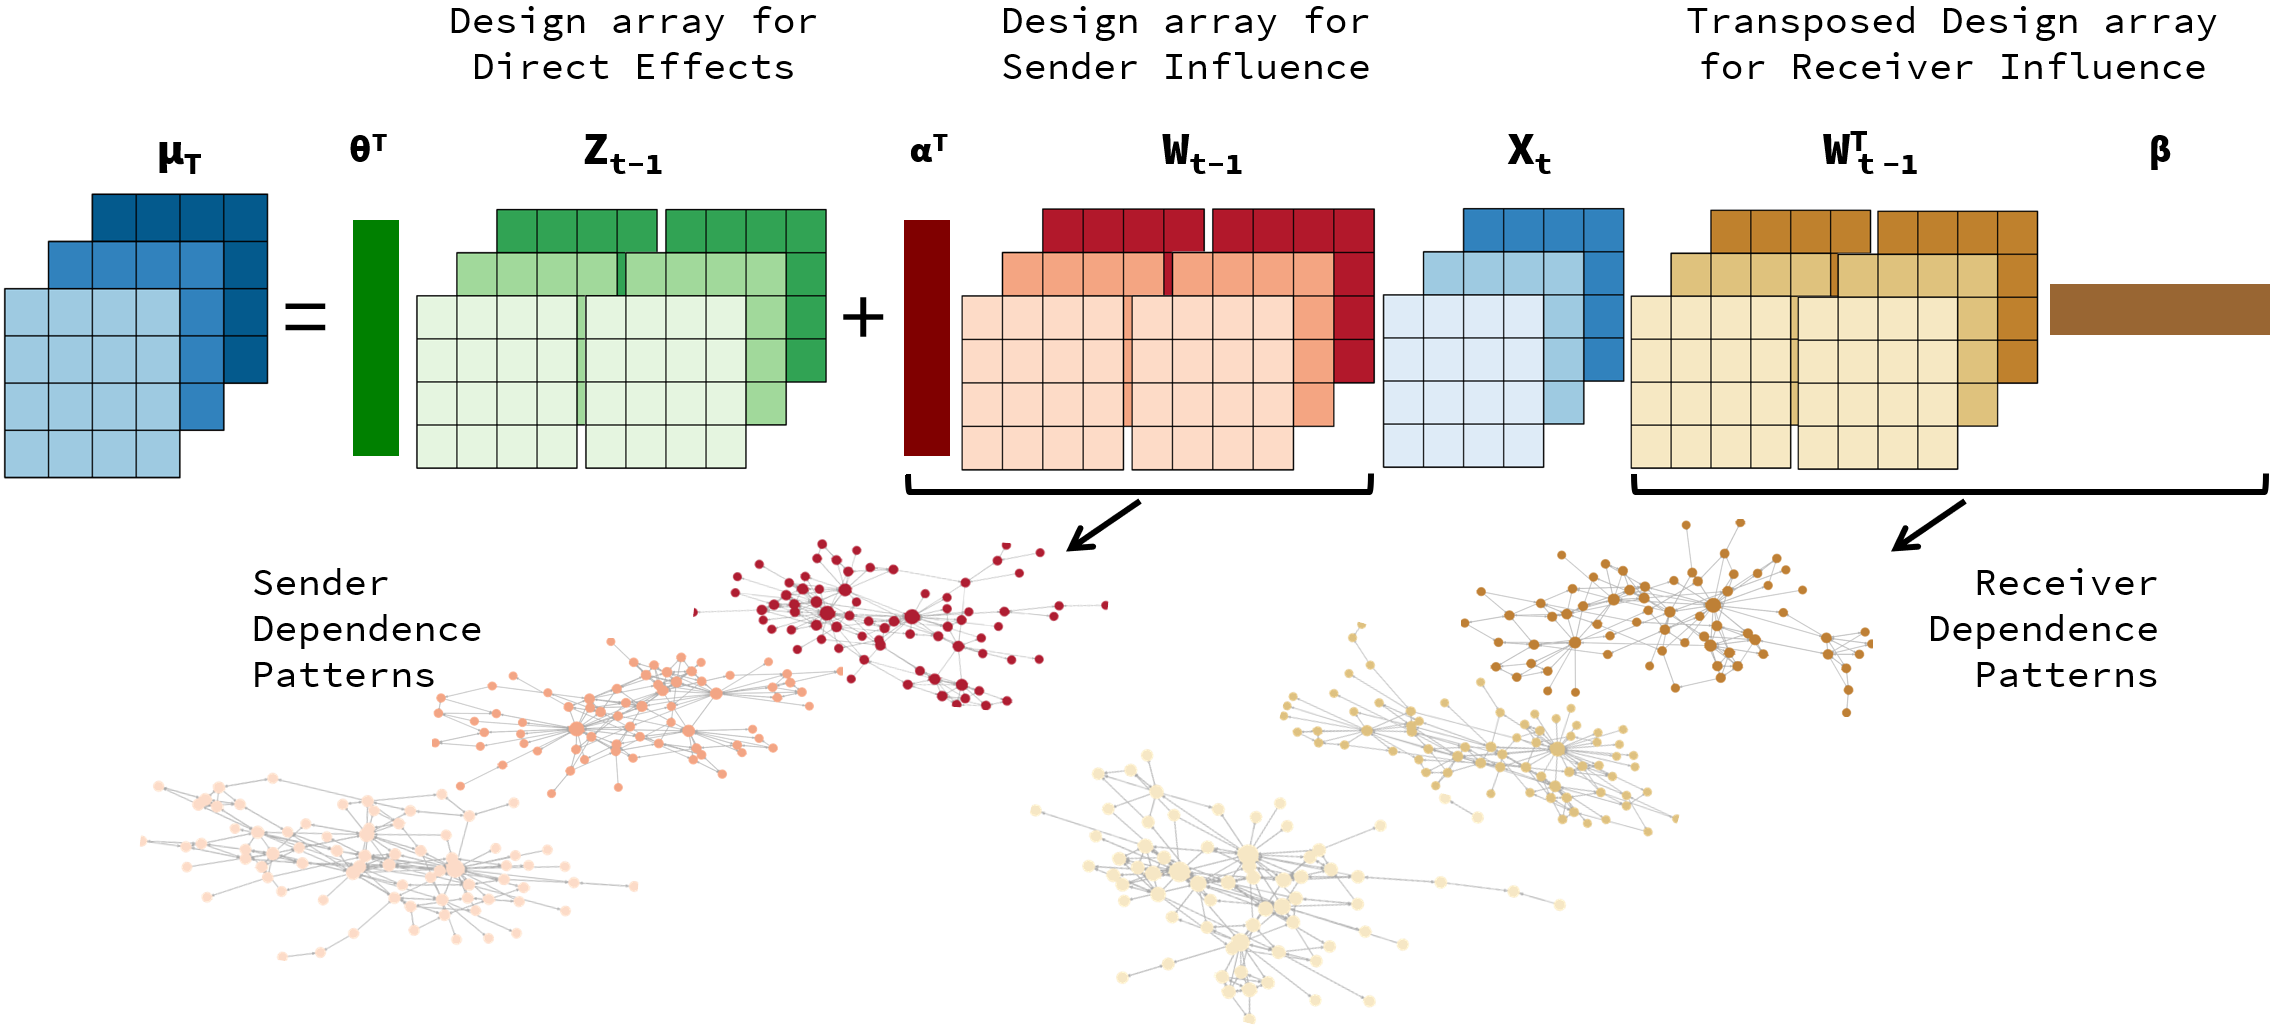
\includegraphics[width=1\textwidth]{socialInfluenceViz3.png}
	\caption{Visual summary of social influence regression model.}
	\label{fig:socialInfluenceViz}
\end{figure}
